\documentclass[12pt,a4paper,titlepage,final]{article}
\usepackage[czech]{babel}
\usepackage[left=1.5cm,text={17cm,24cm},top=2.5cm]{geometry}
\usepackage[utf8]{inputenc}
\usepackage[T1, IL2]{fontenc}
\usepackage{listings}
\lstset{basicstyle=\small\ttfamily}

% Hack: should be placed after hypperref; otherwise, there are no links
\usepackage{multibib}   % Multiple bibliographies
\newcites{My}{Selected Author's Publications}
\usepackage[nottoc]{tocbibind} % Add bibbliographies into ToC

\usepackage{graphicx}   % Enhanced support for graphics
\usepackage{float}      % Figure placing [H]
\usepackage[list=true,listformat=simple]{subcaption} % Captions of multiple figures
 
%\usepackage{multirow}
%\usepackage{dblfloatfix}
\usepackage{booktabs}   % Better-looking tabs
%\usepackage{tabularx}   % Tables
\usepackage{colortbl}   % Cell colors


\newcommand{\myuv}[1]{\quotedblbase #1\textquotedblleft}
\usepackage{url}
\DeclareUrlCommand\url{\def\UrlLeft{<}\def\UrlRight{>} \urlstyle{tt}}
\usepackage{graphicx}
 \usepackage[usenames,x11names,table]{xcolor} % Use colors in listings and figures
\ifx\pdfoutput\undefined % not a pdflatex
\else
	\usepackage[pdftex]{hyperref}
	\hypersetup{
		unicode=true,
		colorlinks=true,
		plainpages=false,
		pdftitle={Retargetable Analysis of Machine Code},
		pdfauthor={Jakub Křoustek},
		pdfsubject={PhD Thesis}, 
		citecolor=DodgerBlue2,
	}
\fi

\begin {document}
\begin{titlepage}
\begin{center}
{\Large\textsc{Fakulta informačních technologií}}\\
{\Large \textsc{Vysoké učení technické v Brně}}\\

\begin{figure}[!h]
 	\centering
	 
\includegraphics[height=7cm]{fit-zp2.pdf}
\end{figure}
\vspace{\stretch{0.382}}

{\Huge 1. Diskrétní simulátor řízený událostmi}\\
\LARGE
IMS projekt\\ 
\vspace{\stretch{0.618}}
\end{center}
{\Large
Vypracovali: Lenka Jalůvková (xjaluv02), Jiří Picek (xpicek01)} \\
{\Large Dne: \today}
\end{titlepage}

%\tableofcontents

\newpage
\section{Úvod} \label{uvod}

V této práci je řešena implementace diskrétního simulátoru pro modelování (\cite{peringer}, slajd 119) založeného na kalendáři událostí (\cite{peringer}, slajd 173). Chování tohoto simulátoru je předvedeno na dvou vybraných příkladech z democvičení předmětu IMS, vybrali jsme příklad Učebna a Kravín (\cite{demo1}, slajd 19 a 22).
Smyslem experimentu je demonstrovat, že náš simulační nástroj \texttt{libsim} odpovídá již existujícím simulátorům.

\subsection{Řešitelé a zdroje informací}

Projekt vypracoval tým ve složení Lenka Jalůvková a Jiří Picek. Využili jsme znalosti nabyté na přednáškách a democvičeních předmětu IMS. Problém jsme také prokonzultovali s doktorem Martinem Hrubým.

\subsection{Experimentální ověřování validity modelu}

Validita vybraných modelů byla ověřena za využití modelů v SIMLIBU odprezentovaných v rámci democvičení předmětu IMS (\cite{priklady}~\texttt{kravin.cpp}, \texttt{ucebna.cpp}). 

Výsledné modely byly testovány na školním serveru merlin.fit.vutbr.cz, systém CentOS a také na notebooku se systémem ArchLinux.
 
\section{Rozbor tématu a použitých metod/technologií}

Diskrétní simulátor modeluje systém jako diskrétní (nespojitou) posloupnost událostí v čase. Diskrétní simulace je tedy opakem simulace spojité, která kontinuálně zaznamenává dynamiku systému v čase. Spojitá simulace může být také označena jako simulace založená na činnostech. Čas je rozdělen na malé intervaly a stav systému je aktualizován na základě množiny činností, které se odehrávají v daném časovém intervalu. Protože diskrétní simulátor nemusí zpracovávat každý časový interval, mohou běžet mnohem rychleji než odpovídající spojité simulátory~\cite{simulace.info}. 

\subsection{Použité postupy}

Diskrétní simulátor je implementován v jazyce C++, který nám umožnil objektový vývoj. Programování nám zjednodušilo využití tříd, které k sobě svazují data a funkce nad nimi.

\subsection{Původ použitých metod/technologií}

Při tvorbě projektu nám byla inspirací knihovna SIMLIB, která umožňuje diskrétní i spojitou simulaci, dále demonstrační cvičení a přednášky předmětu IMS.

\section{Koncepce}

Hlavní komponentou diskrétního simulátoru je kalendář událostí, do kterého přidáváme nebo vyjímáme záznamy. 
Kalendář událostí je uspořádaná datová struktura uchovávající aktivační záznamy budoucích událostí. Každá naplánovaná budoucí událost \emph{next event} má v kalendáři záznam obsahující položky $[(acttime_{i}, priority_{i}, event_{i}), \dots]$. Kalendář umožňuje výběr prvního záznamu s nejnižším aktivačním časem a vkládání/rušení aktivačních záznamů.

Princip kalendáře událostí:
\begin{lstlisting}[label={lst:myListing}]
Inicializace kalendare udalosti a modelu
while(kalendar je neprazdny){
          Vyjmi prvni aktivacni zaznam (AZ) z kalendare
          if (acttime > T_END)
              break; Ukonceni cyklu
         Nastav cas na aktivacni cas acttime v AZ
         Proved popis chovani udalosti event v AZ
}
cas = T_END; konec simulace
\end{lstlisting}

%ještě v koncepci by to chtělo zmínit event a store
Dalšími prostředky pro diskrétní modelování jsou event (báze pro modely událostí) a store (obslužná linka s kapacitou) (\cite{peringer}, slajd 163). Událost je jednorázová akce vyvolaná v určitém modelovém čase. V SIMLIB je odvozena od abstraktní třídy \texttt{Event}, musíme definovat metodu \texttt{Behavior}, jak vidíme níže~\ref{lst:myEvent}. Často jsou nutné periodické události, událost se sama znovu naplánuje. Příklad popisu periodické události:

\begin{lstlisting}[label={lst:myEvent}]
class Udalost : public Event {
    void Behavior() {
        akce udalosti
        Activate(Time + e);  bude se periodicky aktivovat
    }
};
\end{lstlisting}

Store neboli sklad umožňuje simultánní přístup ke zdroji s určitou kapacitou. Event přistupuje ke skladu s požadavkem na obsazení kapacity. Pokud je kapacita volná, přidělí se (zmenší se množství dostupné kapacity), pokud není volná, event čeká ve frontě. Sklad nemá prioritu obsluhy. Kapacitu může vrátit libovolný event. 

\section{Architektura simulačního modelu/simulátoru}

Prvky simulátoru jsou implementovány v pěti hlavních částech (\texttt{event.h}, \texttt{gen.h}, \texttt{libsim.h}, \texttt{stat.h} a \texttt{store.h}), které tvoří prvky našeho simulátoru \texttt{libsim}. Tento simulátor je dále využíván v modelech Kravín a Učebna, které jsou v souborech \texttt{kravin.cpp} a \texttt{ucebna.cpp}. Níže jsou jednotlivé části blíže rozebrány.
 
\subsection{Kalendář událostí}

Kalendář událostí se nachází v souboru \texttt{libsim.h}. Fronta událostí pro kalendář je implementována jako multimapa z knihovny STL (Standard Template Library), která jednotlivé prvky seřadí dle hodnot klíčů, v našem případě časových záznamů. Pokud jsou klíče shodné, jejich pořadí není definováno, to však u simulace není podstatné, protože události se mají provádět ve stejný okamžik, takže nelze rozhodnout, která má přijít dříve.

Hlavní smyčka kalendáře je implementována podle algoritmu výše \ref{lst:myListing} v mírně pozměněném pořadí. Nejprve proběhne kontrola časové zarážky, dále se nastaví čas na čas aktivace aktuální události a poté se vybere událost a zavolá se její provedení. Kalendář se inicializuje pomocí funkce \texttt{init}, které se předává počáteční a koncový čas simulace. Tyto časy je možné kdykoli v simulaci přečíst z proměnných \texttt{TIME} a \texttt{TIME\_END}.

Po ukončení funkce \texttt{run} se kalendář nemaže. Pro smazání se explicitně volá funkce \texttt{freeSimu\-lation}. Statistiky tak můžeme vypisovat ve více časových intervalech.

\subsection{Události}

Další důležitou částí je soubor \texttt{event.h} implementující události v simulaci. Podporují aktivaci v aktuálním čase nebo za zadanou dobu. Události defaultně nemají žádné chování, to se musí vytvořit až v simulaci. 

\subsection{Sklad}

Sklad je implementován v souboru \texttt{store.h}, který obsahuje základní operace se skladem, a to zabrání skladu (metoda \texttt{Enter}) a jeho uvolnění (metoda \texttt{Leave}). Dále obsahuje funkce pro zjištění, zda je sklad prázdný (metoda \texttt{Empty}) či plný (metoda \texttt{Full}). 
 
\subsubsection{Zařízení}
Při použití skladu s defaultními hodnotami parametrů se chová jako zařízení. Jedná se o velikost skladu u konstruktoru a počet zabíraných nebo uvolňovaných míst u \texttt{Enter} a \texttt{Leave}.

\subsection{Generátor}

Generátory jsou implementovány v \texttt{gen.h}. Obsahuje pseudonáhodný generátor čísel z intervalu $\langle$0,1) a dále generátory s exponenciálním, s normálním a rovnoměrným rozložením.

\subsubsection{Pseudonáhodný generátor}

Pseudonáhodný generátor jsme implementovali ve funkci \texttt{Random}, nejprve jsme se inspirovali z opory lineárním kongruentním generátorem (\cite{opora} str. 18-20), avšak generoval příliš malá čísla i s různým nastavením parametrů, čímž nepříznivě ovlivnil výsledky simulací. Nakonec jsme jej implementovali za využití standardní C funkce \texttt{rand}.

\subsubsection{Generátor s exponenciálním rozložením}

Generátor s exponenciálním rozložením je implementován ve funkci \texttt{Exponential}. V tomto případě jsme se inspirovali knihovnou SIMLIB. Pro výpočet využívá výše popsaný pseudonáhodný generátor.

\subsubsection{Generátor s normálním rozložením}

Funkce \texttt{Uniform} obsahuje generátor s normálním rozložením. Funkci jsme implementovali dle principu uvedeného na fóru~\cite{forum}.

\subsubsection{Generátor s rovnoměrným rozložením}

Generátor s rovnoměrným rozložením je implementován ve funkci \texttt{Uniform}. Tuto funkci jsme implementovali na základě předchozích znalostí.

\subsection{Statistiky}

V souboru \texttt{stat.h} jsou implementovány statistiky, jejichž výstup následně můžeme vypsat po dokončení simulace. Statistické výpisy jsou prováděny pouze pro sklad. 

Sledované položky skladu jsou celkový počet požadavků o zabrání skladu, počet požadavků, které zaberou sklad bez čekání ve frontě a statistiky nad frontou u skladu. Sledují se příchozí požadavky ve frontě, dále jeji maximální, průměrná a aktuální délka a minimální, maximální a průměrný čas čekání. 

Funkce statistik se volají v metodách skladu v určitých případech. Pokud se do skladu vstoupí bez čekání ve frontě, zavolá se metoda \texttt{EnterNonqueued} ve které se zvýší počet požadavků o sklad a počet požadavků, které prošly bez fronty. Pokud se vstoupí do fronty, tak se uchová aktuální čas, kdy se vstupuje do fronty, zkontroluje se délka fronty pro uchování maximální délky fronty a zvýší se počet požadavků o sklad. V případě opouštění fronty se dopočítávají minimální, maximální čekací čas a počítá se celkový čas strávený ve frontě, který se při výpisu dále přepočítá na průměrný čas čekání ve frontě.

\subsection{Překlad}

Překlad probíhá pomocí našeho \texttt{Makefile} příkazem \texttt{make ucebna} nebo \texttt{make kravin}, případně lze přeložit a spustit oba příklady najednou pomocí \texttt{make run}. Výsledný překlad je následně umístěn ve složce \texttt{bin}.

\section{Podstata simulačních experimentů a jejich průběh}

Činnost simulátoru byla ověřena na dvou modelech z demonstračních cvičení, a to příklad Učebna a Kravín.

\subsection{Postup experimentování} 

V jednotlivých modelech jsme nejprve nastavili hodnoty parametrů podle příslušných zadání, následně jsme je změnili na základě výsledků. Nakonec jsme je nastavili stejně jako v případě modelů implementovaných pomocí knihovny SIMLIB (\cite{priklady}).

\subsection{Experimenty}

Prováděli jsme experimenty nad oběma příklady (Učebna, Kravín) převzatými z demonstračních cvičení předmětu IMS.

\subsubsection{ Kravín}

První experiment je prováděn při nastavení hodnot shodným se zadáním. V kravíně je 100 krav, 5 dojiček, 1 nakládací rampa a 2 auta. Auto může naložit 20 konvic. Experiment je prováděn v simulačním čase 0 -- 200 hodin.

\begin{figure}[!h] 
 	\centering
	 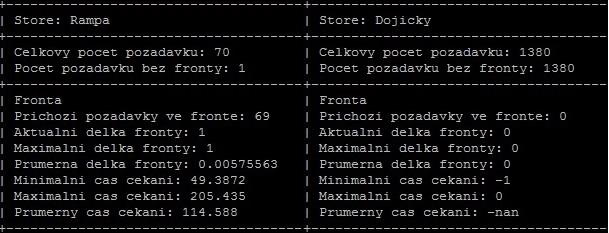
\includegraphics[]{kravy1.jpg}
\caption{Experiment s nastavením dle zadání}
\label{obr1}
\end{figure}

Z výsledku na obrázku~\ref{obr1} vidíme, že dojičky nejsou plně využity. Proto pro další experiment snížíme počet dojiček na 3, stejně jako v simulaci příkladu  SIMLIB (~\cite{priklady}).

\begin{figure}[!h] 
 	\centering
	 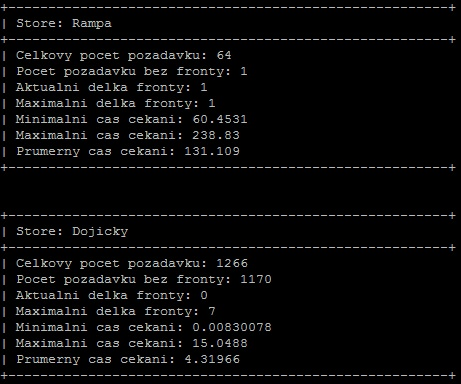
\includegraphics[]{kravy2.jpg}
\caption{Experiment se sníženým počtem dojiček}
\label{obr2}
\end{figure}

Z výsledku na obrázku~\ref{obr2} vidíme, že dojičky jsou lépe využity a že maximálně čekalo 7 krav nejdéle však 15 minut. Dále auto čeká na volnou rampu nejméně hodinu. Naplněné auto náklad převáží maximálně hodinu (30 - 60 minut), proto jsme usoudili, že by mohlo stačit pouze jedno auto, tudíž další experiment je pouze s jedním autem.

\begin{figure}[!h] 
 	\centering
	 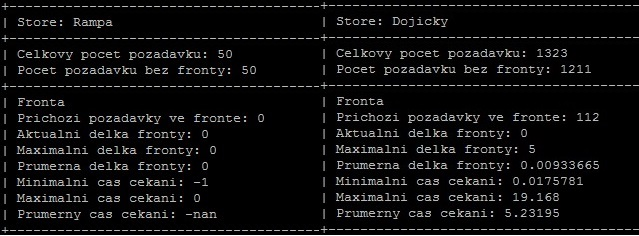
\includegraphics[]{kravy3.jpg}
\caption{Experiment se sníženým počtem aut}
\label{obr3}
\end{figure}

Z výsledků na obrázku~\ref{obr3} vidíme, že auto přepravilo méně konvic než v předchozím případě, vyplatily by se minimálně dvě auta. 

\subsubsection{Učebna}

První experiment je prováděn při nastavení hodnot shodným se zadáním. Máme 10 počítačů, studenti přicházejí v intervalech daných exponenciálním rozložením se středem 10 min. Pokud je počítač volný, obsadí ho a pracují exp(100 min), jinak se 60\% okamžitě postaví do fronty, zbytek odchází. Po 30-60 minutách se však 20\% vrací. Experiment je prováděn v simulačním čase 0 -- 1000000 (stejně jako v demonstračních cvičeních).

\begin{figure}[!h] 
 	\centering
	 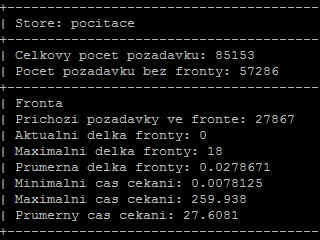
\includegraphics[]{ucebna1.jpg}
\caption{Experiment s nastavením dle zadání}
\label{obr4}
\end{figure}

Z výsledku na obrázku~\ref{obr4} vidíme, že studenti na počítač průměrně čekali 27 min a nejdéle 259 min. Při zvýšení počtu počítačů na 20 se maximální délka výrazně sníží a průměrný čekací čas je také rozumnější, jak vidíme na obrázku~\ref{obr5}.

\begin{figure}[!h] 
 	\centering
	 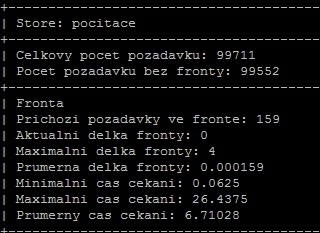
\includegraphics[]{ucebna2.jpg}
\caption{Experiment se zvýšeným počtem počítačů na 20}
\label{obr4}
\end{figure}

Při počtu 25 počítačů se již netvoří fronty vůbec a studenti mohou pracovat bez čekání, jak vidíme na obrázku~\ref{obr5}.

\begin{figure}[!h] 
 	\centering
	 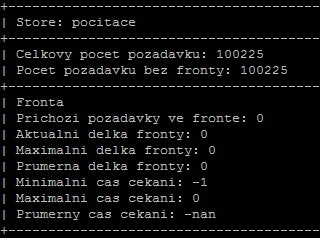
\includegraphics[]{ucebna3.jpg} 
\caption{Experiment se zvýšeným počtem počítačů na 25}
\label{obr5}
\end{figure}

\subsubsection{Závěry experimentů}

Bylo provedeno několik experimentů v různých situacích s rozličným nastavením vstupních parametrů. V průběhu experimentování s Kravínem byla odstraněna chyba v modelu, kdy auto bylo připraveno na rampě,  avšak konvice do něj nebyly nakládány.  Na základě experimentů jsme zjistili, že Kravín by fungoval i v případě 3 dojiček.

V případě Učebny by byla potřeba alespoň 20 počítačů, aby studenti nečekali dlouhé fronty a nejlépe 25, aby mohli pracovat ihned.

%udelat referencni SIMLIB printscreen +ucebna+teorie

\section{Shrnutí simulačních experimentů a závěr}

V rámci projektu vznikl diskrétní simulátor, který byl implementován v C++. Po spuštění vypisujeme statistiky. Implementovali jsme pouze základní z nich, které jsme shledali důležitými, případné další požadavky sledovaných hodnot se dají snadno doplnit.
Ve statistikách je mimo jiné i průměrná délka fronty, která se vždy počítá od času 0, i když čas simulace začíná v jiném čase.

Při experimentování s modelem kravín se naše výsledky oproti výsledkům modelů s knihovnou SIMLIB lišily zhruba o XXX\%. V případě příkladu učebna přibližně o XX\%, jak vidíme v tabulkách~\ref{srovnani} a ~\ref{srovnani2}.

%přepsat nějaké hodnoty do tabulky (např.: sledovaná hodnota (popis) - referenční hodnota - odchylka

\begin{table}[ht]
\caption{Náš simulátor vs. SIMLIB, Kravín se 3 dojičkami, 1 rampou, 2 auty}
\centering
\begin{tabular}{c c c c c}
\hline\hline
& Sledovaná hodnota & náš simulátor & SIMLIB & odchylka\\[0.5ex]
\hline
Rampa & min. čas&  60,453 & 38,4755&\\
 & max. čas & 238,830 & 223,847&\\
 & průměr. čas & 131,109 & 119,114&\\
Dojičky & min. čas & 0,008 & 0,027&\\
 & max. čas & 15,049 & 9,752&\\
 & průměr. čas & 4,312 & 2,878&\\[1ex]
\hline
\label{srovnani}
\end{tabular}
\end{table}

\begin{table}[ht]
\caption{Náš simulátor vs. SIMLIB, Učebna s 10 počítači, studenti exp(10 min)}
\centering
\begin{tabular}{c c c c c}
\hline\hline
& Sledovaná hodnota & náš simulátor & SIMLIB & odchylka\\[0.5ex]
\hline
Počítače & min. čas&  0,008 & 0,003&\\
 & max. čas & 259,938 & 198,401&\\
 & průměr. čas & 27,608 & 28,289&\\[1ex]
\hline
\label{srovnani2}
\end{tabular}
\end{table}

\newpage

\bibliographystyle{myplain}
\bibliography{bibliography}

\end{document}